\documentclass[a4paper,10pt]{article}


\usepackage{project_js}               % package for project documents
\usepackage{shortcuts_js}           % package for shortcuts 


%%%%%%%%%%%%%%%%%%%%%%%%%%%%%%%%%%%%%%%%%%%%%%%%%%
%%%%%%		Début du document 	    %%%%%%
%%%%%%%%%%%%%%%%%%%%%%%%%%%%%%%%%%%%%%%%%%%%%%%%%%




\title{Rédiger un rapport en Latex
}
\author{?, ?, ?, Joseph Salmon}
\date {}


\begin{document}
\sloppy
\maketitle
 % change the glo to an nlo file after the makeindex, idem gls and nls
\tableofcontents 


\newpage
\printnomenclature

\section{Introduction}

Voici un bref aperçu du type de document que l'on peut rédiger avec  Latex.
Ce texte  présente seulement la classe nommée``article'' 
(définie par la commande \lstinline+\usepackage{article}+). 
C'est cette classe  qui vous permettra d'écrire un rapport pour votre projet.


Pour plus d'information et approfondir vos connaissances en Latex, on pourra également consulter   
\href{http://tobi.oetiker.ch/lshort/}{"The not so Short Introduction to LaTeX2e"} de Tobi Oetiker. 
Pour les non anglophiles, la version  en français est disponible  
\href{http://www.laas.fr/~matthieu/cours/latex2e/}{ici}. 
Le site internet \href{http://www.grappa.univ-lille3.fr/FAQ-LaTeX/}{FAQ LaTeX de l'équipe Grappa} 
est lui aussi plein de ressource et répond à la plupart des questions courantes. 
Je conseil aussi le livre sous licence "Art Libre" de Vincent Lozano 
\href{http://www.framabook.org/latex.html}{Tout ce que vous avez toujours voulu savoir sur LaTeX sans jamais oser le demander}.

%%%%%%%%%%%%%%%%%%%%%%%%%%%%%%%%%%%%%%%%%%%%%%%%%%%%%%%%%%%%%%%%%%%%%%%%%%%%%%%%%%%%%%%%%%%%%%%%%%%%%%%%%%%%%%%%%%%%%%%%%%%%%%%%%%%%%%%%%%%%%%%%%%%%%%%%%%%%%%%%%%%%%%%%%%%%%%%%%%%%%%%%%%%%%%%%%%%%%%%%%%%%%%%%%%%%%%%%%%%%%%%%%%%%%%%%%%%%%%%%%%%%%%%%%%%%%%%%


\section{Comment démarrer?}

%%%%%%%%%%%%%%%%%%%%%%%%%%%%%%%%%%%%%%%%%%%%%%%%%%%%%%%%%%%%%%%%%%%%%%%%%%%%%%%%%%%%%%%%%%%%%%%%%%%%%%%%%%%%%%%%%%%%%%%%%%%%%%%%%%%%%%%%%%%%%%%%%%%%%%%%%%%%%%%%%%%%%%%%%%%%%%%%%%%%%%%%%%%%%%%%%%%%%%%%%%%%%%%%%%%%%%%%%%%%%%%%%%%%%%%%%%%%%%%%%%%%%%%%%%%%%%%%

\subsection{Logiciels}
Tout d'abord, il faut disposer d'un éditeur de texte et d'un compilateur.

\begin{itemize}
\item Sous Mac : installer MacTex  (éditeur + compilateur) . L'éditeur s'appelle Texshop.  
\item Sous Linux : Latex est installé de base, il vous faut juste un bon éditeur. Kile est très bien et largement suffisant
dans un premier temps. Les experts pourront utiliser Vim ou emacs. 
\item Sous Windows : installer Miktex d'abord (chercher avec un moteur de recherche) puis Texniccenter ou  Winshell par exemple.
\end{itemize}

%%%%%%%%%%%%%%%%%%%%%%%%%%%%%%%%%%%%%%%%%%%%%%%%%%%%%%%%%%%%%%%%%%%%%%%%%%%%%%%%%%%%%%%%%%%%%%%%%%%%%%%%%%%%%%%%%%%%%%%%%%%%%%%%%%%%%%%%%%%%%%%%%%%%%%%%%%%%%%%%%%%%%%%%%%%%%%%%%%%%%%%%%%%%%%%%%%%%%%%%%%%%%%%%%%%%%%%%%%%%%%%%%%%%%%%%%%%%%%%%%%%%%%%%%%%%%%%%

\subsection{Format de fichier et compilation}





En Latex, on écrit un code ``barbare'' qui sera compil\'e par un programme. Sur vos terminaux c'est Kile qui compilera : il faut aller dans l'onglet ``\textbf{build}'' ou ``\textbf{construire}'', puis cliquer sur ``\textbf{compile}''. On choisit alors le type de compilation (Latex, pdfLatex, bibtex pour la bibliographie \ldots). 
Si en sortie on veut un fichier ps : il faut faire ``\textbf{tex to dvi}'' puis  ``\textbf{dvi to ps}''
Si en sortie on veut un fichier pdf : il faut faire ``\textbf{pdfLatex}'' (mieux pour afficher des documents avec des hyperliens et des images de formats standards).

Le fichier Latex du document que vous êtes en train de lire est  disponible ici : \href{http://people.math.jussieu.fr/~salmon/enseignement/M1/introlatex.tex}{ceci est un lien hypertexte}.  Son extension est  .tex. Une fois le fichier compilé,  on obtiendra un ``joli'' document en format .pdf ou bien .ps. Pour visualiser le résultat il suffit d'aller dans l'onglet  ``\textbf{build}'' (ou constuire), choisir ``\textbf{view}`` (ou voir) puis de sélectionner ``\textbf{Viewpdf}'' (si l'on a fait pdfLatex).\medskip

Ceci fait, on choisit la classe de document  que l'on veut créer.  Pour les projets,  la classe ``\textbf{article}'' est recommandée (les élèves motivés qui voudraient écrire un livre entier pourront utiliser la classe ``\textbf{book}''). Le document commence donc par la commande :\medskip

\begin{lstlisting}
\documentclass[a4paper,12pt]{article}
\end{lstlisting}

Les options d'une fonction Latex sont toujours entre crochets. Ici elles déterminent le format (A4) du document, et définissent la taille de la police (12pt).\medskip


\subsection{Les Packages}

En dessous du choix de la classe on donne la définition des packages que l'on veut utiliser. Les packages sont des bibliothèques utilisées pour des fonctions avancées, que l'on doit charger. Par exemple la commande  \lstinline+\usepackage{amsmath}+ charge le package ``\textbf{asmath}'', qui est utile  pour écrire des symboles mathématiques. Le package ``\textbf{babel}''  est lui utilisé pour écrire des accents (du moins avec l'option ``\textbf{french}''). En effet, les anglophones n'en ont pas besoin, donc initialement Latex ne gère pas les accents. L'intérêt du package est donc de pallier ce manque. \medskip

Les packages sont des fichiers au format .sty. Ils sont pour la plupart déjà installés sur votre ordinateur (par Miktex ou Texshop). Par contre, il se peut que certains packages ne soient pas disponibles.  Pour les rendre utilisables pour la compilation il suffit de télécharger le fichier ``\textbf{***.sty}''  sur internet (on les trouvera sur le site du  \href{http://www.ctan.org/}{CTAN})  et de le placer dans le dossier où vous éditez votre fichier .tex.     \medskip

\subsection{Formules Mathématiques et Théorèmes}
On peut définir des environnements comme des théorèmes, des propositions, etc. par les commandes :\medskip
\begin{lstlisting}
\newtheorem{theorem}{Theorem}[section] 
\newtheorem{prop}[theorem]{Proposition}\medskip
\end{lstlisting}
Cela donne :

\begin{theorem}
 L'ensemble des nombres premiers est infini.
\end{theorem}
Les théorèmes  sont ainsi numérotés par Latex de manière automatique.

\begin{theorem}
 L'ensemble des nombres premiers congrus à 1 modulo 4 est infini.
\end{theorem}

\begin{proof}
 ici on ferait la démonstration ... mais  je vous la laisse en exercice.
\end{proof}



Une fois les packages définis, on peut créer des raccourcis pour les quantités qui reviennent souvent ou des fonctions. Ici on définit un raccourcis pour la commande qui permet de créer une fonction :\medskip

\lstinline+\newcommand{\nc}{\newcommand}+

\begin{rem}
 Toutes les fonctions (au sens informatique du terme) connues par Latex commencent par $\backslash$ (backslash) comme par exemple \lstinline+\sum+
 qui permet d'afficher le symbole de sommation $\sum_{i=1}^{4}$. 
\end{rem}


Pour les formules Mathématiques, on doit  les mettre entre deux signes 
$\$$ pour qu'elles soit interprétées comme des commandes spéciales et non comme du texte. 
Pour écrire le signe de sommation ci-dessus on écrit donc \lstinline+$\sum\_{i=1}^{4}$+ dans le fichier .tex. Si l'on veut afficher des calculs sur une ligne à part on peut par exemple écrire 

\[\mathcal{S}f = \sum_{k\in\mathbb{Z}} \hat f[k] e^{i2\pi kt/T} \] 

en mettant cette fois les formules  entre  les commandes 
\lstinline+\[+ et \lstinline+\]+. On peut aussi utiliser un environnement qui commence par la commande 
\lstinline+\begin{blabla}+ et finit par la commande \lstinline+\end{blabla}+. Si blabla= align, 
on peut aligner des calculs facilement:
\begin{align}
 \mathcal{S}f & = \sum_{k\in\mathbb{Z}} \hat f[k] e^{i2\pi kt/T} \label{nomformule}\\
  & = \sum_{k\in\mathbb{Z}} \hat f[k] e^{i2\pi kt/T}
\end{align}

\begin{rem}
On notera que la numérotation s'est déclenchée toute seule pour les formules. 
On peut  leur donner des noms avec la commande label,  dont la syntaxe est  \lstinline+\label{nomformule}+.  
On s'y réfère plus tard dans le document  avec la commande \lstinline+\ref{nomformule}+. 
Ainsi l'ordre des équations peut être changé sans avoir besoin de renuméroter tout un document. 
Notre première équation est donc \ref{nomformule}. 
Si l'on ne veut pas numéroter une équation,  on met une étoile à la fin de l'environnement 
(écrire \lstinline+align*+ à la place d'\lstinline+align+ par exemple).
\end{rem}



Pour un grand panel de symboles mathématiques, il suffit de regarder les raccourcis fournis par l'éditeur que vous utilisez ou de chercher sur Internet un lexique. Voici néanmoins quelques commandes : pour aller à la ligne  $\backslash\backslash$ , 
pour une nouvelle feuille \lstinline+\newpage+, pour les trois points  \lstinline+\ldots+\medskip
\\
On renvoit à \href{http://www.ctan.org/get/info/symbols/comprehensive/symbols-a4.pdf}{``The Comprehensive Latex Symbol List''} par Scott Pakin pour une liste exhaustive de tous les symboles connus.


%%%%%%%%%%%%%%%%%%%%%%%%%%%%%%%%%%%%%%%%%%%%%%%%%%%%%%%%%%%%%%%%%%%%%%%%%%%%%%%%%%%%%%%%%%%%%%%%%%%%%%%%%%%%%%%%%%%%%%%%%%%%%%%%%%%%%%%%%%%%%%%%%%%%%%%%%%%%%%%%%%%%%%%%%%%%%%%%%%%%%%%%%%%%%%%%%%%%%%%%%%%%%%%%%%%%%%%%%%%%%%%%%%%%%%%%%%%%%%%%%%%%%%%%%%%%%%%%


\subsection{Organisation du document}
On commence par donner un titre au  fichier, le nom de l'auteur et éventuellement la date par les commandes suivantes :\medskip
\begin{lstlisting}
\title{Faire un rapport en Latex} 
\author{Joseph Salmon} 
\date{ }
\end{lstlisting}

Ensuite on commence le corps du document avec \lstinline+\begin{document}+ 
(ne pas oublier de fermer tout en bas du document par la commande \lstinline+\end{document}+). 
On insère le titre avec \lstinline+\maketitle+ et la table des matières avec \lstinline+\tableofcontents+.
La construction de la table des matières se fait automatiquement. 
Elle donne l'arborescence du document, dans l'ordre où les chapitres et sous chapitres sont donnés 
dans le fichier .tex.\medskip	


On crée  des chapitres, sous chapitres en écrivant simplement  au début d'un chapitre \lstinline+\section{Le nom du chapitre}+ 
et pour les sous-chapitres \lstinline+\subsection{Le nom du sous chapitre}+.  
Latex numérote tout seul les chapitres dans l'ordre où ils se présentent. 
Si l'on intervertit deux chapitres, à la prochaine compilation les numéros seront automatiquement échangés. Il faut parfois deux compilations pour afficher correctement la table des matières.  \medskip
 
Ceci fait vous pouvez déjà commencer à rédiger un premier document, visuellement correcte avec toutes les formules de mathématiques dont vous avez besoin. Au chapitre suivant on va voir quelques raffinements possibles pour égayer vos documents.

%%%%%%%%%%%%%%%%%%%%%%%%%%%%%%%%%%%%%%%%%%%%%%%%%%%%%%%%%%%%%%%%%%%%%%%%%%%%%%%%%%%%%%%%%%%%%%%%%%%%%%%%%%%%%%%%%%%%%%%%%%%%%%%%%%%%%%%%%%%%%%%%%%%%%%%%%%%%%%%%%%%%%%%%%%%%%%%%%%%%%%%%%%%%%%%%%%%%%%%%%%%%%%%%%%%%%%%%%%%%%%%%%%%%%%%%%%%%%%%%%%%%%%%%%%%%%%%%

\section{Opérations spéciales}


%%%%%%%%%%%%%%%%%%%%%%%%%%%%%%%%%%%%%%%%%%%%%%%%%%%%%%%%%%%%%%%%%%%%%%%%%%%%%%%%%%%%%%%%%%%%%%%%%%%%%%%%%%%%%%%%%%%%%%%%%%%%%%%%%%%%%%%%%%%%%%%%%%%%%%%%%%%%%%%%%%%%%%%%%%%%%%%%%%%%%%%%%%%%%%%%%%%%%%%%%%%%%%%%%%%%%%%%%%%%%%%%%%%%%%%%%%%%%%%%%%%%%%%%%%%%%%%%

\subsection{Insérer une image }

Après avoir créé des graphiques avec Scilab, Matlab ou tout autre logiciel,  vous pouvez avoir envie de les insérer dans votre rapport. Cette opération est plus compliquée qu'avec un éditeur de texte classique. Voici le code pour insérer l'image ci-dessous : \medskip

\begin{lstlisting}
\begin{figure}[htb]
\begin{minipage}[b]{0.48\linewidth}
\centering
\centerline{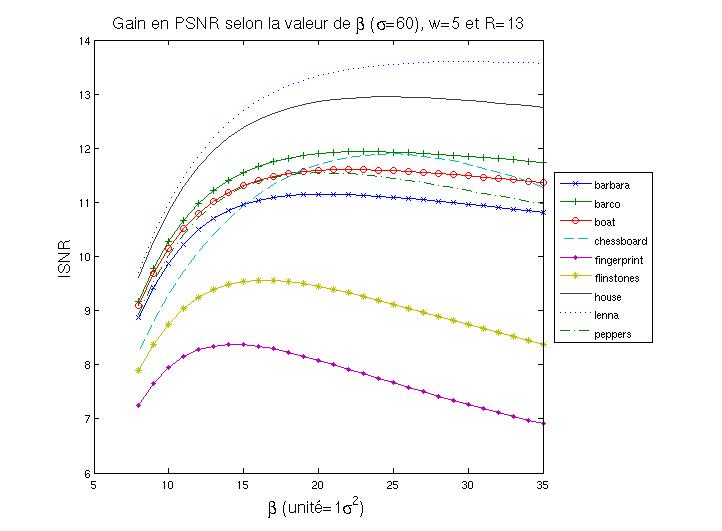
\includegraphics[width=1.44\ textwidth]{psnr_sig60.jpg}}
\vspace{0.1cm}
\centerline{(A) un premier graphique}
\medskip
\end{minipage}
\hfill
\begin{minipage}[b]{.48\linewidth}
\centering
\centerline{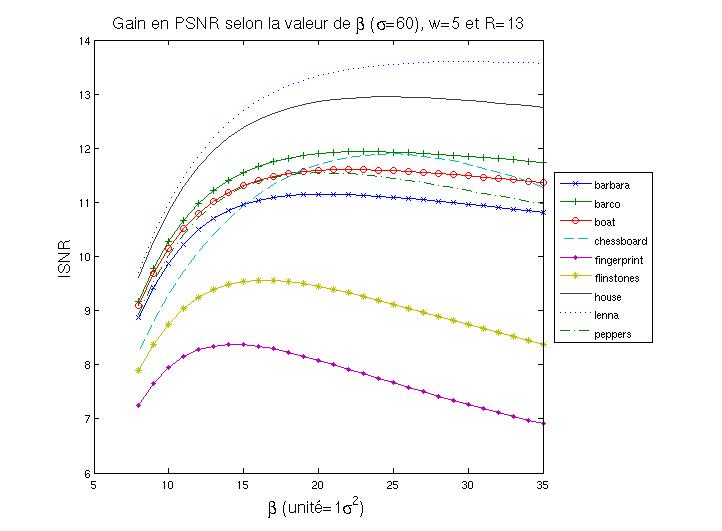
\includegraphics[width=1.44\ textwidth]{psnr_sig60.jpg}}
\vspace{0.1cm}
\centerline{(B) un autre}
\end{minipage} 
\caption{Des graphiques encore des graphiques...}
\label{fig:ma\_figure}
\end{figure}
\end{lstlisting} 

\medskip
\begin{figure}[htb]
\begin{minipage}[b]{0.48\linewidth}
  \centering
 \centerline{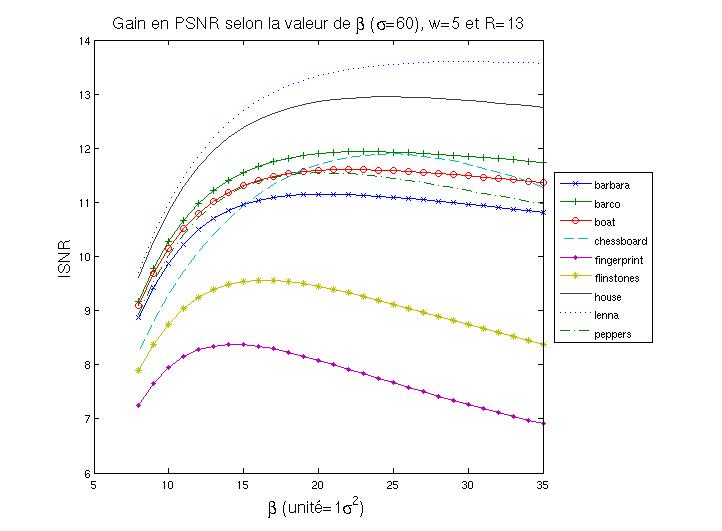
\includegraphics[width=1.44\textwidth]{psnr_sig60.jpg}}
  \vspace{0.1cm}
  \centerline{(A) un premier graphique }\medskip
\end{minipage}
\hfill
\begin{minipage}[b]{.48\linewidth}
  \centering
 \centerline{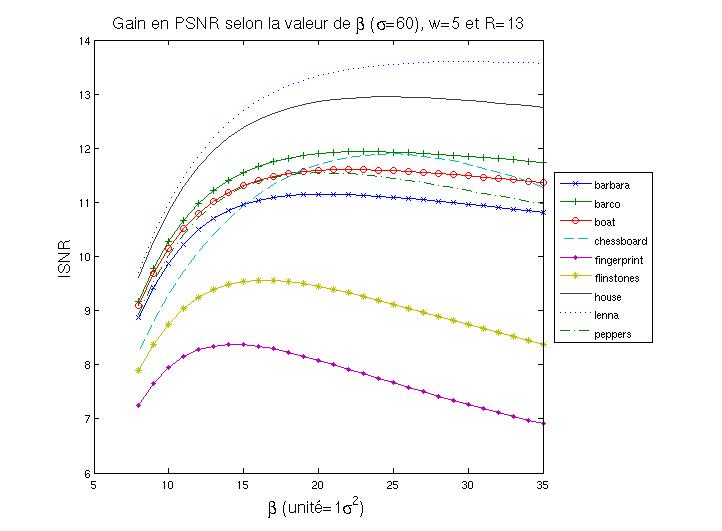
\includegraphics[width=1.44\textwidth]{psnr_sig60.jpg}}
  \vspace{0.1cm}
  \centerline{(B) un deuxième graphique}\medskip
\end{minipage}%

\caption{Des graphiques encore des graphiques...mais quand m\^eme le .jpg c'est bien nul	}
\label{fig:ma_figure}
\end{figure}

L'image insérée doit se trouver par défaut dans le même répertoire où se trouve le fichier .tex que vous écrivez. On pourra faire varier les paramètres de taille pour voir comment jouer sur la taille de l'image que l'on insère. Il existe d'autres façons d'insérer des images, mais celle-ci à l'avantage de bien fonctionner \ldots \medskip


En ''pdfLatex'' (version largement conseillée)  on peut insérer des images au format .jpg, .png, .pdf \ldots En revanche, si l'on compile pour obtenir un fichier .ps avec ``\textbf{Latex}'' il faut insérer des fichiers sous le format (peu connu) .eps. Les commandes en revanche ne diffèrent pas.\medskip

Grâce au label utilisé pour la figure, on peut se référer  à celle-ci comme pour les équations, par la commande \lstinline+\ref{fig:ma_figure}+. Ansi la première figure est la figure \ref{fig:ma_figure}.

\subsection{Liens hypertextes}

Pour ce faire il faut utiliser les packages pdftex et hyperref.
On insère un lien hypertexte par la commande \lstinline+\url+\nomenclature[A]{$\backslash$url}{$\backslash$url} si l'on veut écrire un lien hypertexte présentant le site cible. 
Par exemple on peut trouver de l'aide sur latex sur le site officiel : 
\url{http://www.ctan.org/} (la commande est \lstinline+\url{http://www.ctan.org/}+). 
Mais on peut aussi le faire avec  \lstinline+\href+, qui permet de définir n'importe quel mot comme lien. 
Par exemple \href{http://www.ctan.org/}{là} se trouve le site donné ci-dessus 
(avec la commande : \lstinline+\href{http://www.ctan.org/}{adresse}+).  
Les références, citations, entrées de la table des matières sont directement hypertextes 
(c.-à-d qu'on peut cliquer dessus pour aller à l'emplacement correspondant).
On pourra utiliser la ligne suivante pour définir divers packages utiles  d'un seul coup :
\begin{lstlisting}
\usepackage[pdftex,a4paper,linkcolor=test,citecolor=vertsombre,colorlinks=true, 
      pagebackref,bookmarks=true, plainpages=true,urlcolor=freeblue]{hyperref}
\end{lstlisting}

\subsection{Insérer un algorithme}
Plutôt que de donner un fichier de programmation, il peut être utile d'introduire dans son document un schéma de l'algorithme que l'on a utilisé. Pour cela, on peut choisir les packages suivants :\medskip

\begin{lstlisting}
\usepackage{algpseudocode}
\usepackage{algorithm} 
\usepackage{algpascal}
\end{lstlisting}

On peut alors obtenir  l'exemple suivant :\medskip 

\alglanguage{pseudocode}
\begin{algorithmic}[1]
\Procedure{EW-Aggregate}{$(P(Y))$,$\sigma$}  
\State $H=0;$
   \While{$H <T$} 
      \State$\lambda \gets \lambda+h/T \times L;$
	\EndWhile\label{euclidendwhile}
   \State \textbf{return} $\lambda$ 
\EndProcedure
\end{algorithmic}
\medskip

Les commandes utilisées sont :
\begin{lstlisting}
\alglanguage{pseudocode}
\begin{algorithmic}[1]
\Procedure{EW-Aggregate}\{$(P(Y))$,$\sigma$}  
\State\$H=0;\$
\While{\$H <T\$} 
\State\lambda\gets\lambda+h/T\times L;
\EndWhile\label\{euclidendwhile}
\State\textbf\{return} $\lambda$ 
\EndProcedure
\end{algorithmic}
\end{lstlisting}
\noindent Pour plus de détail sur ce package :\medskip

\noindent\url{www.ctan.org/get/macros/latex/contrib/algorithmicx/algorithmicx.pdf}

%%%%%%%%%%%%%%%%%%%%%%%%%%%%%%%%%%%%%%%%%%%%%%%%%%%%%%%%%%%%%%%%%%%%%%%%%%%%%%%%%%%%%%%%%%%%%%%%%%%%%%%%%%%%%%%%%%%%%%%%%%%%%%%%%%%%%%%%%%%%%%%%%%%%%%%%%%%%%%%%%%%%%%%%%%%%%%%%%%%%%%%%%%%%%%%%%%%%%%%%%%%%%%%%%%%%%%%%%%%%%%%%%%%%%%%%%%%%%%%%%%%%%%%%%%%%%%%%

\section{Bibliographie}


Pour les références bibliographiques,  il faut créer un autre fichier d'extension .bib, qui est l'extension des fichiers ``\textbf{bibtex}''. On le met également dans le dossier qui contient le fichier .tex que l'on rédige. Le fichier de la bibliographie associée à ce document est disponible \href{http://people.math.jussieu.fr/~salmon/enseignement/M1/refs.bib}{là}.  On présente les articles, livres et autres sites webs de la façon suivante : (on peut trouver également ce type d'information tout rempli sur internet, comme sur le site \href{http://ams.u-strasbg.fr/mathscinet/}{MathSciNet} par exemple.)\medskip
\begin{lstlisting}
@inproceedings{Tsybakov03, 
  author    = {A. B. Tsybakov},
  title     = {Optimal Rates of Aggregation}, 
  booktitle = {COLT}, 
  year      = {2003}, 
  pages     = {303-313}, 
  bibsource = {DBLP, http://dblp.uni-trier.de}, 
}
\end{lstlisting}

On doit alors compiler la bibliographie avec la commande bibtex. Il faut aller dans l'onglet ``\textbf{build}'' ou ``\textbf{construire}'', puis cliquer sur ``\textbf{compile}''. Le type de compilation est alors Bibtex.\medskip

La citation apparaît à l'endroit voulu grâce à la commande  \lstinline+\ref{nom citation}+. 
Tout à la fin du fichier .pdf, on trouve alors  les références voulues avec tous les détails que l'on a précisés 
sur le document cité. 
Pour cela il faut  écrire juste avant \lstinline+\end{document}+ les commandes 
\lstinline+\bibliography{nom du fichier de la bibliographie}+
\lstinline+\bibliographystyle{alpha}+ pour que les citations apparaissent avec des lettres et l'année et non juste des numéros. Par exemple on peut parler de l'article \cite{Tsybakov03} ou bien du livre \cite{Catoni04}. Les articles non cités n'apparaissent pas. \medskip

On remarquera qu'à la fin de la bibliographie, les pages où une référence est citée apparaissent sous forme de liens hypertextes. C'est l'utilisation du package ``\textbf{pagebackref}'' qui rend cela possible.
Pour plus d'informations sur Bibtex en français : 
\href{http://www.irit.fr/~Gael.Jaffre/LOGICIELS/LATEX_BIBTEX/bibtex1.html}{Le site de Gaël Jaffré},
\href{http://fr.wikipedia.org/wiki/BibTeX}{Wikipedia},  
et en anglais :  \href{http://www.bibtex.org/}{www.bibtex.org} 


%%%%%%%%%%%%%%%%%%%%%%%%%%%%%%%%%%%%%%%%%%%%%%%%%%%%%%%%%%%%%%%%%%%%%%%%%%%%%%%%%%%%%%%%%%%%%%%%%%%%%%%%%%%%%%%%%%%%%%%%%%%%%%%%%%%%%%%%%%%%%%%%%%%%%%%%%%%%%%%%%%%%%%%%%%%%%%%%%%%%%%%%%%%%%%%%%%%%%%%%%%%%%%%%%%%%%%%%%%%%%%%%%%%%%%%%%%%%%%%%%%%%%%%%%%%%%%%%

\newpage
\appendix
\begin{center}
    {\bf ANNEXE}
  \end{center}
Enfin avec la commande \lstinline+\appendix+, on crée un chapitre à part dans lequel la numération est distincte du corps du document.
\section{Démonstrations }
Ici on peut mettre en appendice des calculs trop longs. 
\section{Programmes}
Ici on peut mettre les programmes informatiques que l'on a rédigés \ldots
\section{Fin}
Voilà bonne rédaction !




%%%%%%%%%%%%%%%%%%%%%%%%%%%%%%%%%%%%%%%%%%%%%%%%%%%%%%%%%%%%%%%%%%%%%%%%%%%%%%%%%%%%%%%%%%%%%%%%%%%%%%%%%%%%%%%%%%%%%%%%%%%%%%%%%%%%%%%%%%%%%%%%%%%%%%%%%%%%%%%%%%%%%%%%%%%%%%%%%%%%%%%%%%%%%%%%%%%%%%%%%%%%%%%%%%%%%%%%%%%%%%%%%%%%%%%%%%%%%%%%%%%%%%%%%%%%%%%%
\printnomenclature

\clearpage
% \addcontentsline{toc}{chapter}{Bibliographie}
\bibliographystyle{plainnat}
%\bibliographystyle{plain}
\bibliography{refs}
\end{document}